\documentclass[12pt,a4paper]{article}
\usepackage{vntex} % Tiếng Việt
\usepackage{graphicx} % Chèn hình ảnh
\usepackage{listings} % Thêm gói listings để chèn code
\usepackage{xcolor} % Màu cho code
\usepackage{changepage} % Thay đổi lề
\lstset{
    language=R,
    basicstyle=\footnotesize\ttfamily,
    numbers=none,
    numberstyle=\tiny\color{gray},
    stepnumber=1,
    numbersep=0.01pt,
    tabsize=2,
    breaklines=true,
    breakatwhitespace=false,
    xleftmargin=0cm, % for line numbers
    framexleftmargin=0cm, % for code frame
    keywordstyle=\color{blue},
    commentstyle=\color{green},
    stringstyle=\color{orange},
    frame=single,
    rulecolor=\color{black},
    basicstyle=\ttfamily,
}
% Thiết lập bảng
\usepackage{diagbox}
\usepackage{array}
\usepackage{tabularx}
\usepackage{longtable} % Tạo bảng qua nhiều trang
\usepackage{cellspace}
\usepackage{bm} % Chữ in đậm trong công thức toán 
\usepackage{a4wide,amssymb,epsfig,latexsym,multicol,array,hhline,fancyhdr}
\usepackage{tikz}
\usepackage{color}
\usepackage{subcaption}
\usepackage{framed}
\usepackage{float} % Để chèn hình ảnh vào đúng vị trí
\usepackage{fancyvrb} %Đưa dữ liệu dạng nguyên thủy vào
\usepackage{amsmath} % Công thức toán
\usepackage{slashbox} % Chèn đường chéo trong bảng
% Thiết lập kích thước
\usepackage{geometry}
\geometry{
    left=3cm,
    right=2cm,
    top=2.5cm,
    bottom=2.5cm,
}
\usepackage{hyperref} %Chèn link
\hypersetup{urlcolor=black,linkcolor=black,citecolor=black,colorlinks=true} % Màu cho các đường nét
\everymath{\color{black}}
\setlength{\headheight}{40pt}
\pagestyle{fancy}


%Header
\fancyhead{} % clear all header fields
\fancyhead[L]{
 \begin{tabular}{rl}
    \begin{picture}(25,15)(0,0)
    \put(0,-8){
\includegraphics[width=12mm, height=12mm]{pictures/hcmut.png}}
    %\put(0,-8){\epsfig{width=10mm,figure=hcmut.eps}}
   \end{picture}&
	%
\includegraphics[width=8mm, height=8mm]{hcmut.png} & %
	\begin{tabular}{l}
		\textbf{\bf \ttfamily Trường Đại Học Bách Khoa - ĐHQG TP.Hồ Chí Minh}\\
		\textbf{\bf \ttfamily Khoa Cơ Khí - Bộ môn Cơ Điện Tử}
	\end{tabular} 	
 \end{tabular}
}
\fancyhead[R]{
	{\tiny \bf \quad} % Khoảng trắng nhỏ trong header bên phải
}

%Footer
\fancyfoot{} % clear all footer fields
\fancyfoot[L]{\scriptsize \ttfamily Trang bị điện - điện tử trong máy công nghiệp}
\fancyfoot[R]{\scriptsize \ttfamily Trang {\thepage}/13}
\renewcommand{\headrulewidth}{0.3pt}
\renewcommand{\footrulewidth}{0.3pt}

\begin{document}
    \begin{titlepage}   
    \begin{center}
        \vspace*{-2cm} 
        \large
        \textbf{ĐẠI HỌC QUỐC GIA THÀNH PHỐ HỒ CHÍ MINH \\
        TRƯỜNG ĐẠI HỌC BÁCH KHOA\\
        KHOA CƠ KHÍ\\
        BỘ MÔN CƠ ĐIỆN TỬ}\\
        
\includegraphics[width=70mm, height=70mm]{pictures/hcmut.png} \\
        \rule{\linewidth}{0.5mm}\\
        \vspace{0.8cm}
        \Large
        \textbf{TRANG BỊ ĐIỆN - ĐIỆN TỬ TRONG MÁY CÔNG NGHIỆP}\\
        \vspace*{0.5cm}
        \Huge
        \textbf{EXERCISE 3}\\
        \vspace{0.5cm}
        \rule{\linewidth}{0.5mm}\\
        \vspace{0.8cm}
        \vspace{1cm}
        \large
        GVHD: TS. LÊ ĐỨC HẠNH\\
        \vspace{0.5cm}
        DANH SÁCH THÀNH VIÊN:\\[0.3cm]
        \begin{tabular}{|>{\centering\arraybackslash}m{1cm}|>{\centering\arraybackslash}m{7cm}|>{\centering\arraybackslash}m{5cm}|}
            \hline
            \textbf{STT} & \textbf{Họ và tên} & \textbf{MSSV} \\
            \hline
            1 & Võ Hữu Dư & 2210604 \\
            \hline
            2 & Dương Quang Duy & 2210497 \\
            \hline
            3 & Trần Quang Đạo & 2210647 \\
            \hline
        \end{tabular}
    \end{center}
        
    \vfill
    \large
    \begin{center}
        TP.HCM, \today
    \end{center}
\end{titlepage}

	\tableofcontents
	\newpage
 	\section{For the below figure}
    \begin{figure}[H]
        \centering
        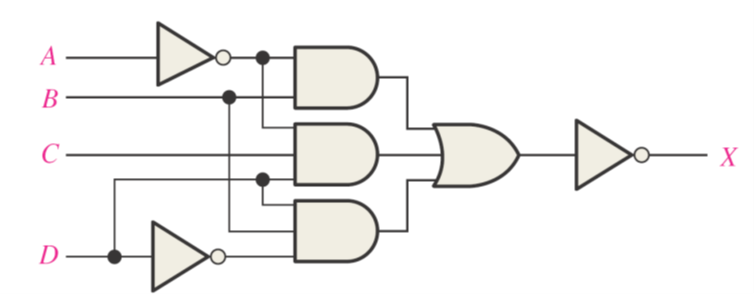
\includegraphics[width=0.5\textwidth]{pictures/1_diagram.png}
        \caption{Sơ đồ mạch bài 1}
    \end{figure}
    \subsection{Derive the output and minimize the output function using Karnaugh map}
        \hspace*{0.6cm}Từ sơ đồ mạch ta có giá trị đầu ra:
        \begin{align*}
            X(A, B, C, D) &= \overline{(\bar{A} \cdot B) + (\bar{A} \cdot C \cdot D) + (B \cdot D \cdot \bar{D})} \\
            &= \overline{(\bar{A} \cdot B) + (\bar{A} \cdot C \cdot D)}  
        \end{align*}
        \hspace*{0.6cm}Rút gọn biểu thức bằng bìa Karnaugh:
        \begin{align*}
            X(A, B, C, D) &= \overline{(01)(01 + 10 + 01 + 00) + 0(0 + 1) (11)} \\
            &= \overline{0111 + 0110 + 0101 + 0100 + 0011 + 0111} \\
            &= \overline{\sum{(7,6,5,4,3)}} = \sum{(0,1,2,8,9,10,11,12,13,14,15)} \\
        \end{align*}
        \hspace*{0.6cm}Vậy ta có bảng Karnaugh và biểu thức rút gọn:
        \begin{figure}[H]
            \centering
            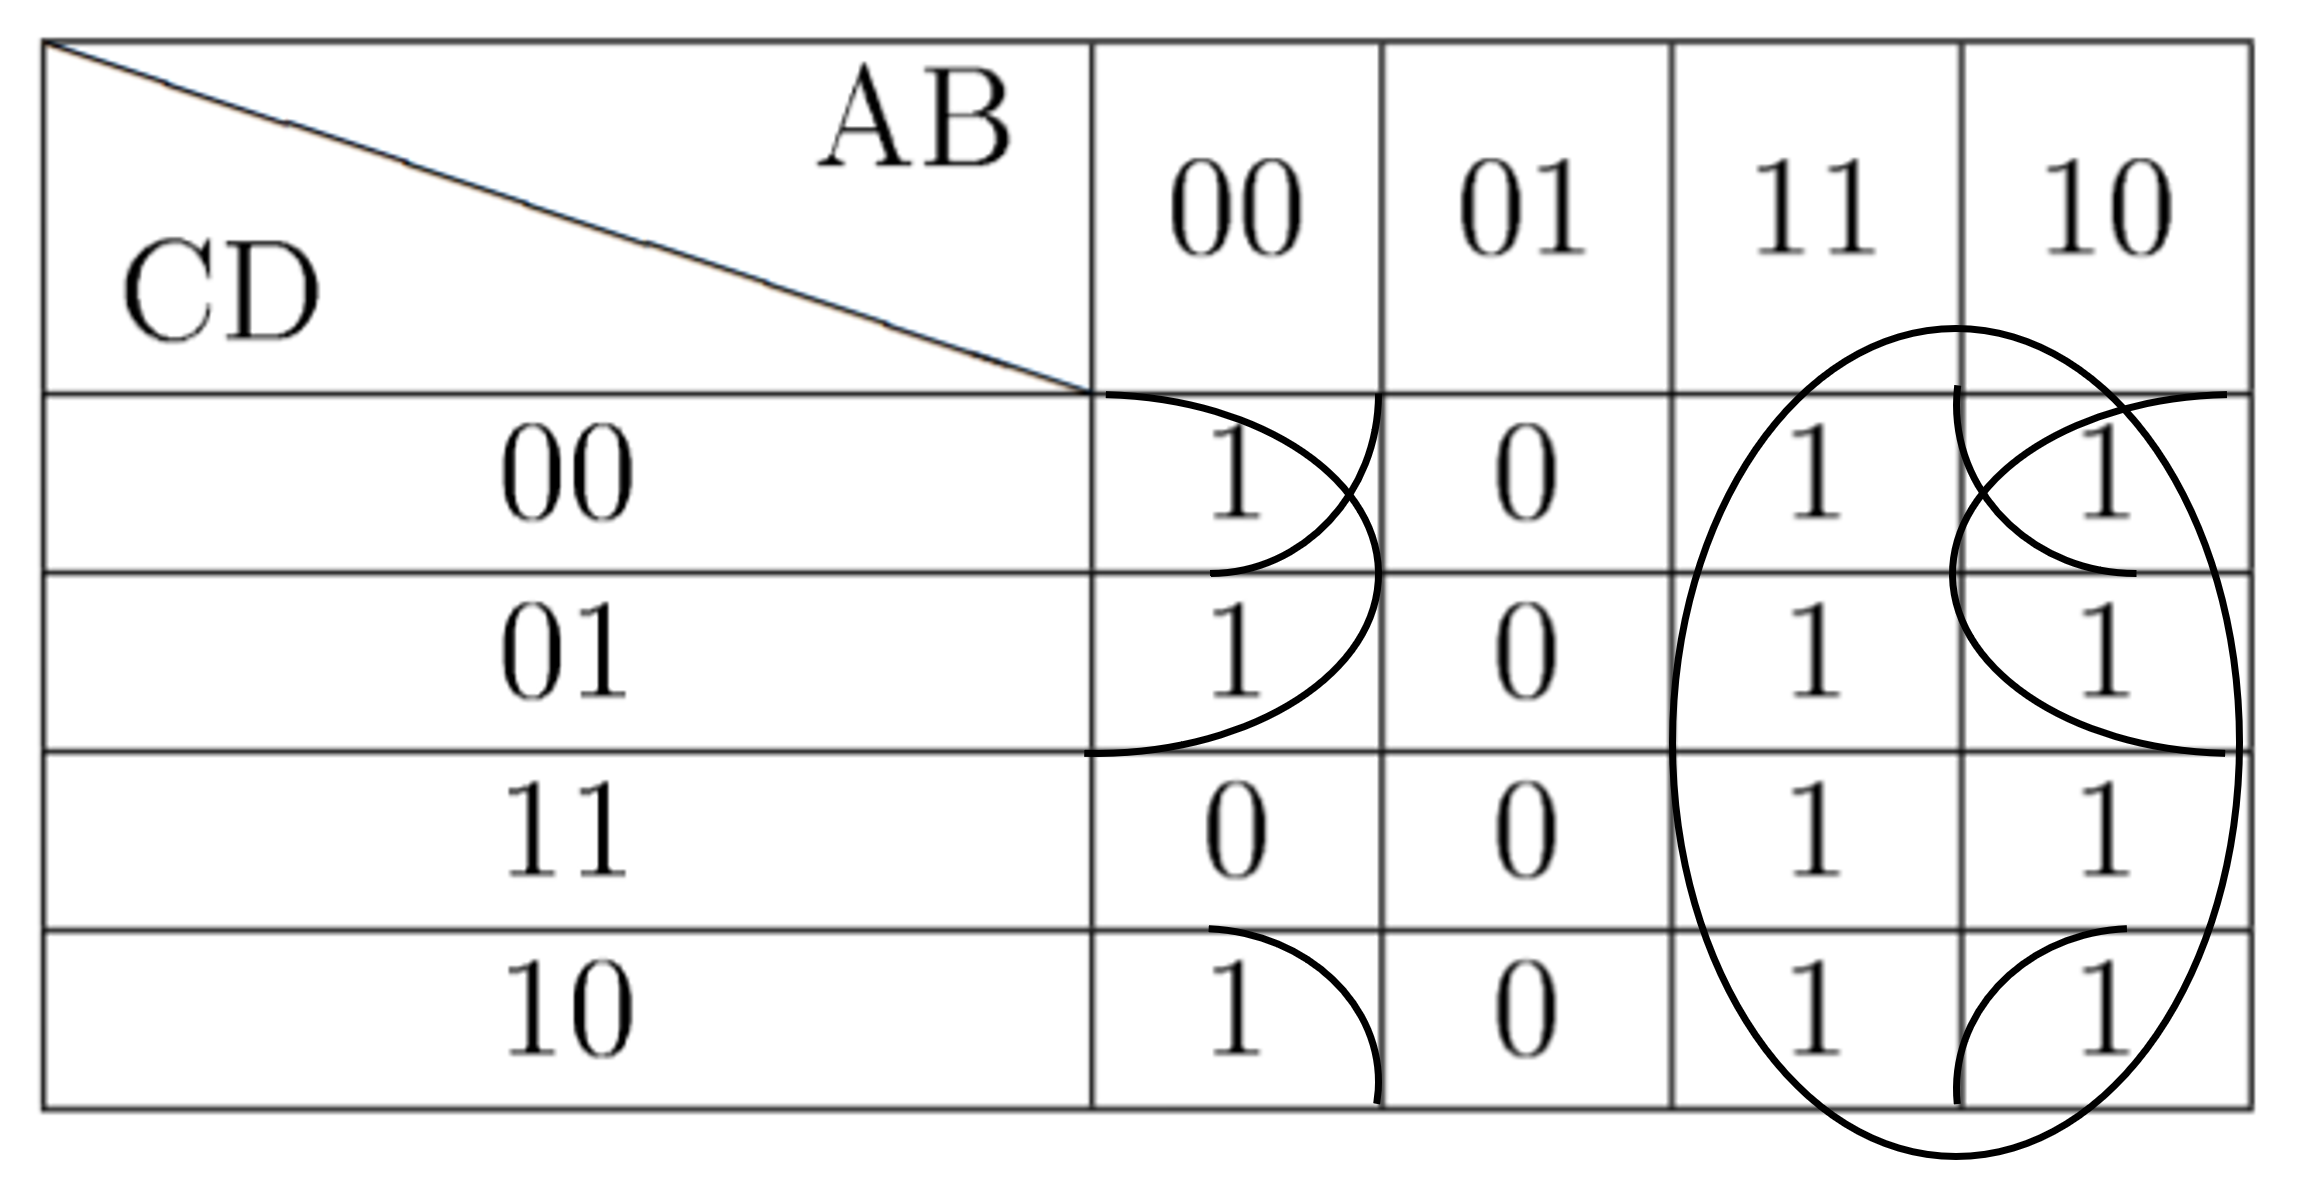
\includegraphics[width=0.5\textwidth]{pictures/1_karnaugh.png}
            \caption{Bảng Karnaugh bài 1}
        \end{figure}
        Từ bảng Karnaugh ta có biểu thức rút gọn:
        \begin{align*}
            X(A, B, C, D) &= \sum{(0,1,2,8,9,10,11,12,13,14,15)} = \bar{B}\bar{C} + \bar{B}\bar{D} + A\\
        \end{align*}
    \subsection{Draw the wave form of output if}
        \begin{figure}[H]
            \centering
            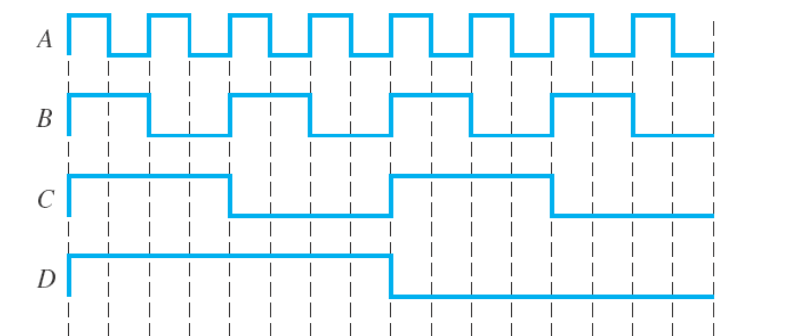
\includegraphics[width=0.8\textwidth]{pictures/1_waveinput.png}
            \caption{Waveform input bài 1}
            \label{fig:1_waveinput}
        \end{figure}
        \hspace*{0.6cm}Từ biểu thức rút gọn và đầu vào như hình \ref{fig:1_waveinput} ta có đầu ra như hình \ref{fig:1_waveoutput}
        \begin{figure}[H]
            \centering
            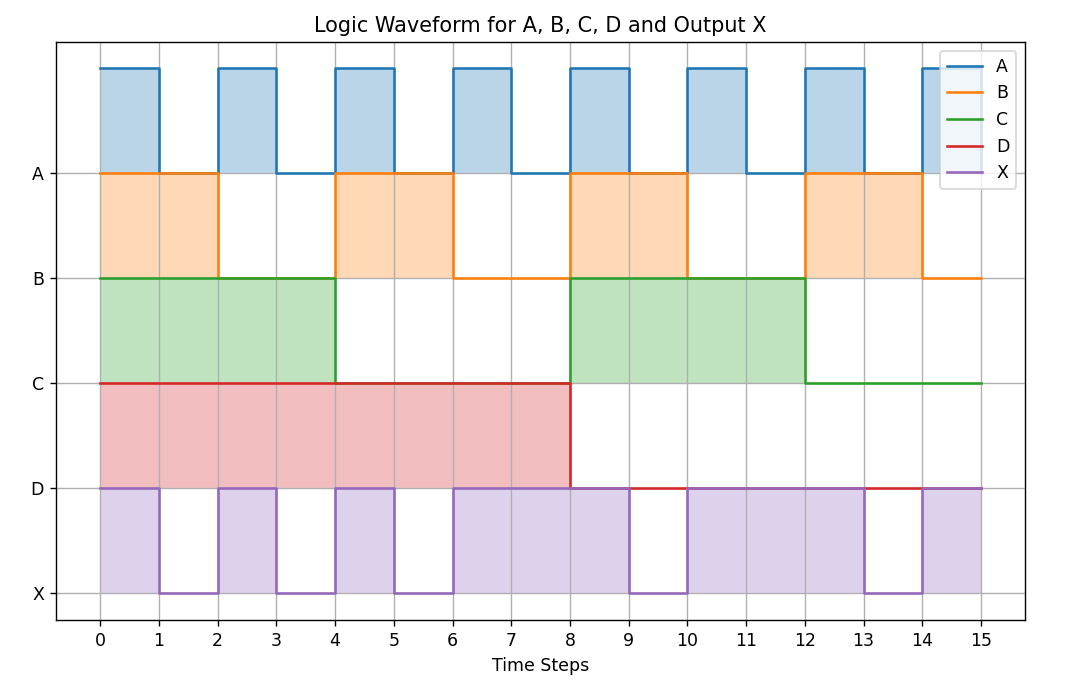
\includegraphics[width=0.8\textwidth]{pictures/1_waveoutput.png}
            \caption{Waveform output bài 1}
            \label{fig:1_waveoutput}
        \end{figure}
        
\end{document}